\documentclass[conference]{IEEEtran}
\IEEEoverridecommandlockouts
\usepackage{cite}
\usepackage{amsmath,amssymb,amsfonts}
\usepackage{graphicx}
\usepackage{booktabs}
\usepackage{hyperref}
\usepackage{tabularx}

\begin{document}

\title{TransitRisk: Cost-Sensitive, Calibrated Next-Hour Delay Risk Forecasting for Urban Transit Operations}

\author{\IEEEauthorblockN{Ayush, Manav, Parth}
\IEEEauthorblockA{DATA 245 Machine Learning Technologies}}

\maketitle

\begin{abstract}
Urban transit systems regularly experience delay spillovers that degrade reliability and increase both passenger and operator burden. This paper presents TransitRisk, an end-to-end machine learning system for predicting next-hour elevated delay risk at the station-route-hour level. The implemented pipeline includes synthetic data generation, preprocessing, temporal feature engineering, model training, calibration, threshold optimization, uncertainty estimation, and dashboard deployment. The dataset starts from approximately 1.25 million trip events and aggregates to approximately 153 thousand station-route-hour records. Seven candidate classifiers are evaluated, and calibrated XGBoost is selected for deployment. On held-out test data, the final model achieves ROC-AUC 0.810, PR-AUC 0.766, F1 0.643, and Brier score 0.169 (from saved metrics artifact). A cost-sensitive threshold policy with C(FN)=5 and C(FP)=1 yields t\_cost \approx 0.163 (from saved thresholds artifact). Conformal prediction is integrated to expose uncertainty in operator-facing views. The resulting dashboard supports risk monitoring, what-if analysis, threshold tuning, stress slicing, explainability, and live replay simulation.
\end{abstract}

\begin{IEEEkeywords}
Transit delay forecasting, cost-sensitive learning, calibration, conformal prediction, XGBoost, decision support dashboard
\end{IEEEkeywords}

\section{Introduction}
Transit delay is operationally costly because disruptions propagate across routes, stations, and time windows. Simple rule-based thresholds and short-horizon heuristics often fail under dynamic weather and demand conditions. TransitRisk addresses this gap with an end-to-end ML system that predicts whether a station-route pair will experience elevated delay in the next hour and converts risk estimates into actionable decisions.

Contributions include: (i) a complete pipeline from synthetic generation to deployment, (ii) strict temporal splitting with leakage checks, (iii) 38-feature engineering across temporal, lag, weather, and interaction categories, (iv) calibration and cost-sensitive threshold optimization, and (v) conformal uncertainty integrated into a production dashboard.

\section{Dataset Description}
The project uses synthetic but structured transit data to preserve reproducibility while representing realistic delay dynamics. The dataset contains approximately 1.25M trip events and approximately 153K station-route-hour aggregated rows. Target definition is binary: next-hour elevated delay if mean delay is at least 5 minutes. Main training artifacts and dashboard inputs are produced from strict chronological ordering (60/20/20 train/validation/test) exported as split indices.

\section{Data Preprocessing}
Processing includes timestamp normalization, schema checks, aggregation from trip-level to station-route-hour, missing-value handling, and leakage prevention via temporal alignment. Features at time $t$ are computed from current/past information only, while labels correspond to $t+1$ outcomes. Temporal split boundaries are validated in the feature-engineering stage before indices are exported for downstream modeling and dashboard evaluation.

\section{Proposed Framework}
Problem formulation predicts $\hat{p}_{t+1}=P(y_{t+1}=1\mid x_t)$ for each station-route-hour instance. The pipeline consists of data generation, aggregation, feature engineering, temporal split, model training, calibration, cost-sensitive threshold optimization, conformal uncertainty, evaluation, and dashboard deployment.

Model set: Logistic Regression, Naive Bayes, kNN, Decision Tree, Random Forest, SVM-RBF, and XGBoost. Final deployment uses a saved calibrated XGBoost artifact with threshold policy: $t_{default}=0.50$, $t_{F1}\approx0.345$, $t_{cost}\approx0.163$ under $C_{FN}=5$, $C_{FP}=1$.

\begin{table}[htbp]
\caption{Feature-group summary used in TransitRisk.}
\label{tab:feature_groups}
\centering
\renewcommand{\arraystretch}{1.15}
\begin{tabularx}{\linewidth}{@{}l c X@{}}
\toprule
\textbf{Group} & \textbf{Count} & \textbf{Representative Features} \\
\midrule
Time signals & 8 &
hour sin/cos, day-of-week sin/cos, is\_weekend, peak-morning/evening flags, month \\

Current state & 6 &
mean\_delay, std\_delay, share\_delayed\_5, trip\_count, headway, demand \\

Delay history & 10 &
lag\_1h/2h/3h, rolling\_6h mean/std, same-hour-yesterday and same-hour-last-week \\

Weather & 7 &
temperature, precipitation, wind, visibility, precip\_lag\_1h, precip\_rolling\_3h, wind\_lag\_1h \\

Interactions & 3 &
peak$\times$precip, short\_headway$\times$demand, weekend$\times$precip \\

Spatial/context & 4 &
target-encoded station/route IDs, business quartiles \\
\bottomrule
\end{tabularx}
\end{table}

\section{Workflow Diagram}
\begin{figure}[htbp]
\centering
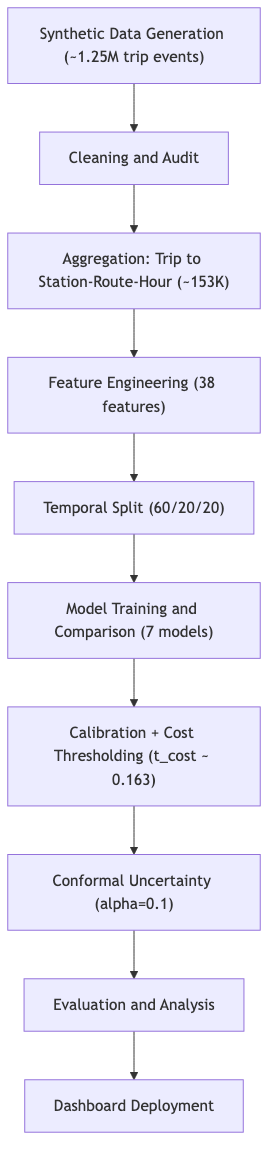
\includegraphics[width=\linewidth]{diagrams/workflow.png}
\caption{End-to-end workflow of TransitRisk from data generation to dashboard deployment.}
\label{fig:workflow}
\end{figure}

\section{Experimental Design}
Chronological validation is used to avoid temporal leakage. Metrics include ROC-AUC, PR-AUC, F1, and Brier score. PR-AUC is emphasized due to class imbalance and alerting context. Reported table values are taken directly from the saved \texttt{figures/metrics.json} artifact used by the dashboard.

\section{Experimental Results}
\begin{table}[htbp]
\caption{Held-out test performance (from saved metrics artifact).}
\label{tab:results}
\centering
\begin{tabular}{lcccc}
\toprule
Model & ROC-AUC & PR-AUC & F1 & Brier \\
\midrule
Logistic Regression & 0.7601 & 0.6764 & 0.5998 & 0.1916 \\
Naive Bayes & 0.7083 & 0.5743 & 0.4887 & 0.2614 \\
kNN & 0.7757 & 0.7185 & 0.5837 & 0.1851 \\
Decision Tree & 0.7849 & 0.7249 & 0.5916 & 0.1782 \\
Random Forest & 0.8061 & 0.7618 & 0.6691 & 0.1766 \\
\textbf{XGBoost (Final)} & \textbf{0.8097} & \textbf{0.7662} & 0.6433 & \textbf{0.1691} \\
SVM-RBF & 0.7534 & 0.6994 & 0.5853 & 0.1916 \\
\bottomrule
\end{tabular}
\end{table}

XGBoost provides the strongest combined ranking performance and probability quality, making it most suitable for calibrated risk-based decisioning in deployment. This checkpoint reflects implemented components only; additional ablation and error-slice analysis are planned for final submission.

\section{System Architecture}
\begin{figure}[htbp]
\centering
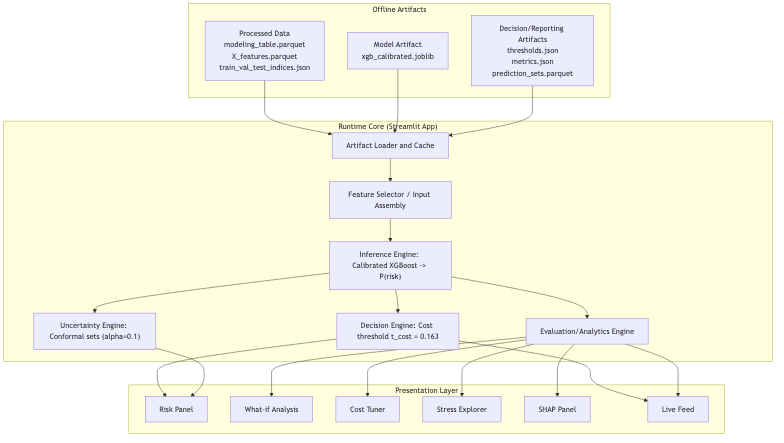
\includegraphics[width=\linewidth]{diagrams/architecture.png}
\caption{TransitRisk system architecture: artifacts, runtime inference core, decision/uncertainty layers, and dashboard modules.}
\label{fig:architecture}
\end{figure}

\section{Work Distribution}
Ayush: synthetic data design, aggregation, preprocessing QA.\\
Manav: model development, dashboard integration, end-to-end deployment.\\
Parth: calibration, thresholding, conformal uncertainty, reporting and analysis.

\section{Conclusion}
TransitRisk demonstrates a full ML-to-operations pipeline for next-hour transit delay risk. The deployed system combines calibrated probabilistic forecasting, cost-aware decision policy, and uncertainty-aware interpretation in a practical dashboard. Future work includes live GTFS integration, online recalibration, and drift-aware updates.

\bibliographystyle{IEEEtran}
\begin{thebibliography}{00}
\bibitem{xgb} T. Chen and C. Guestrin, ``XGBoost: A Scalable Tree Boosting System,'' KDD, 2016.
\bibitem{platt} J. Platt, ``Probabilistic Outputs for Support Vector Machines,'' 1999.
\bibitem{conformal} V. Vovk, A. Gammerman, and G. Shafer, \textit{Algorithmic Learning in a Random World}, 2005.
\end{thebibliography}

\end{document}
